% !TeX spellcheck = en_US
% !TeX root = ../build/users-fees.tex
% !TeX TXS-program:compile = txs:///xelatex/[--shell-escape]



\section{User Fees Flows}

In this section, we will delve into the economic process that starts when a user wants to send some transaction to the L2 network. Our discussion will be split into two parts: firstly, the transaction flow done by the \textbf{RPC} until it is dispatched by the user, concluding when it is stored in the \textbf{Pool}. Secondly, we will examine the sequence transaction flow managed by the \textbf{Sequencer}, ending in some execution.

\subsection{RPC Flow}

The \textbf{RPC} is the zkEVM component that, in a high level, handles the acceptance or rejection of incoming transactions and saves the approved transactions in the \textbf{Pool}. In Figure \ref{fig:rpc-flow}, the transaction progression within the \textbf{RPC} component is shown, starting from the moment a user is willing to send a transaction to the network to the point where it becomes either stored in the \textbf{Pool} or rejected. Let's examine the Figure \ref{fig:rpc-flow} in detail.


\begin{figure}[H]
\centering
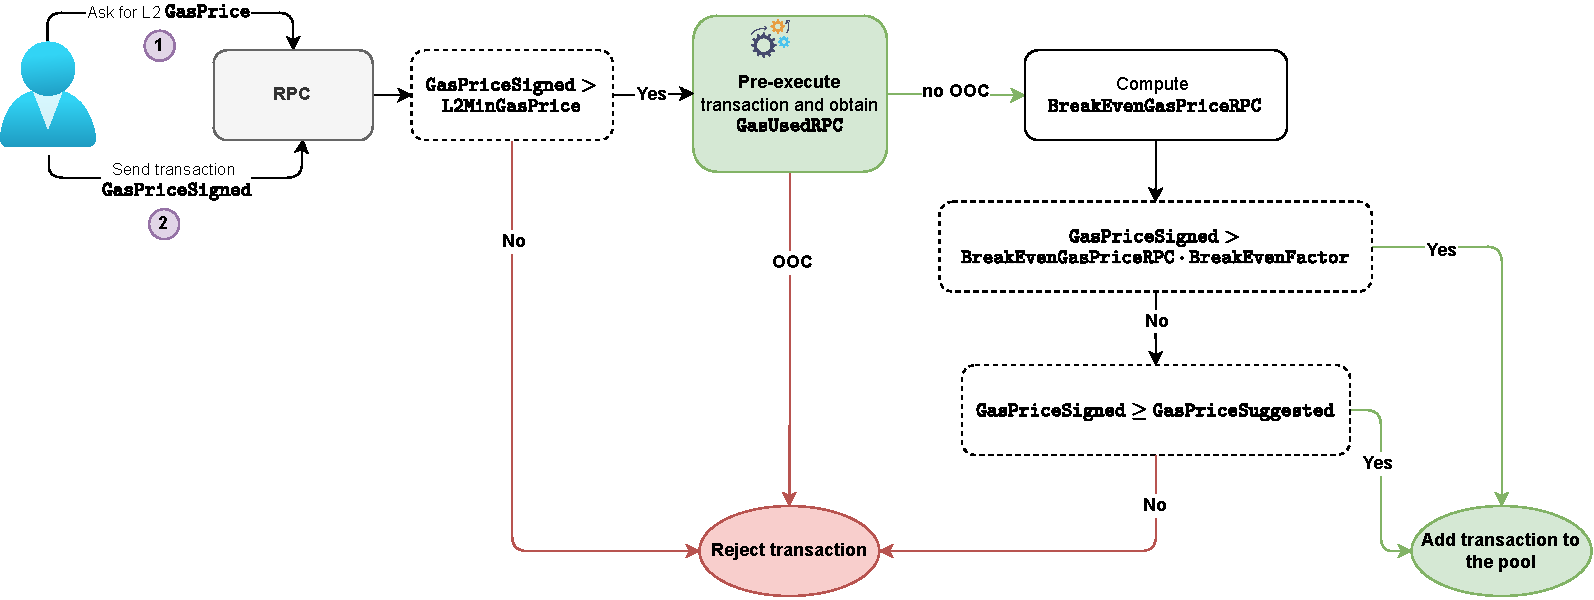
\includegraphics[width=0.9\textwidth]{\zkevmdir/figures/architecture/economics-users-fees/rpc-diagram.drawio}
\caption{Flow of a transaction within the \textbf{RPC} component. As a result of this flow, a transaction can be either included in the \textbf{Pool} for future sequencing or rejected from the network. }
\label{fig:rpc-flow}
\end{figure}

\begin{enumerate}

\item First of all, the users asks to the \textbf{RPC} for the current \texttt{GasPriceSuggested}, which recall is a factor of the current L1 \texttt{GasPrice}. More concretely,
\[
\texttt{GasPriceSuggested} = \texttt{L1GasPrice} \cdot \texttt{SuggestedFactor},
\]
where \texttt{SuggestedFactor} (which is currently of $0.15$) satisfies
\[
\texttt{SuggestedFactor} > \texttt{L1GasPriceFactor}
\]
in order to be able to cover data availability costs. Observe that the suggested gas price varies over time as \texttt{L1GasPrice} also does.

\item Now, the user sends the transaction selecting a \texttt{GasPriceSigned}, the same as in L1. Observe that, from asking for a suggested gas price to sending the transaction has passed some unbounded period of time, where the L1 Gas Price could have increased. Henceforth, rejecting a transaction if $\texttt{GasPriceSigned} < \texttt{GasPriceSuggested}$ does not offer a good user experience. In contrast, we give a margin of $5$ minutes (controlled by the \texttt{MinAllowedGasPriceInterval} parameter). If the signed gas price does not strictly exceed \texttt{MinL2GasPrice}, which is the minumum suggested gas price of $5$ minutes before sending the transaction refreshed every $5$ seconds (controlled by the \texttt{IntervalToRefreshGasPrices} parameter),
\[
\texttt{GasPriceSigned} > \texttt{L2MinGasPrice},
\]
we automatically \textbf{reject} the transaction, since it will not be possible to cover costs.

\item If the transaction was not rejected in the previous step, the RPC uses a cloud executor in order to pre-execute the transaction. Observe that this pre-execution is only an estimated execution since the used state root is not the correct one, as the transaction has not been sequenced yet. Recall that once a transaction is added into the \textbf{Pool}, it is mandatory that it is eventually sequenced. Due to this fact, the purpose of this is to filter transactions according and estimate a fair gas price in an early processing stage, to avoid future losses. As a result of this pre-execution it is obtained and estimated amount of used Gas, which will be called \texttt{GasUsedRPC}. If by pre-executing the transaction we run out of counters, we immediately \textbf{reject} the transaction.

\item If the transaction was not reverted due to \textbf{OOC error}, we compute the current break even gas price, which we will call \texttt{BreakEvenGasPriceRPC}. Recall that it depends on the current \texttt{L1GasPrice}, the transaction size, the \texttt{GasUsed RPC} and a parameter \texttt{NetProfit} that is present in order to include the network's profit for the whole transaction's processing.

\item Now, we have two different paths:

\begin{itemize}

\item If the gas price signed by the user at the time of sending the transaction is higher than the \texttt{BreakEvenGasPriceRPC}, increased by a factor $\texttt{BreakEvenFactor} \geq 1$ (and currently set at $1.3$) used to protect the network against bad Gas usage estimations in the RPC
\[
\texttt{GasPriceSigned} > \texttt{BreakEvenGasPriceRPC} \cdot \texttt{BreakEvenFactor}
\]
then the transaction is immediately \textbf{accepted} and stored in the pool.

\item Otherwise, if
\[
\texttt{GasPriceSigned} \leq \texttt{BreakEvenGasPriceRPC} \cdot \texttt{BreakEvenFactor}
\]
we are in dangerous zone because we may be facing losings due high data availability costs or to fluctuation between future computations, so we \textbf{should reject} the transaction. However, we are currently not directly rejecting transactions in this case.

\end{itemize}

\item In the later case, we check if the gas price signed with the transaction exceeds the current suggested gas price:
\[
\texttt{GasPriceSigned} \geq \texttt{GasPriceSuggested}.
\]
In this case, we take the risk of possible losses, sponsoring the difference if necessary and we introduce the transaction into the \textbf{Pool}. However, if $\texttt{GasPriceSigned} < \texttt{GasPriceSuggested}$ we assume that is highly probable that we face losing and we immediately reject the transaction.

\end{enumerate}


\paragraph*{Final Considerations}

It is important to remark that, as we have said before, once a transaction is included into the pool, we should actually sequence it, that is, we should include it into a block. Hence, if something goes bad in later steps and the gas consumption deviates significantly from the initial estimate, we risk incurring losses with no means to rectify the situation. On the contrary, if the process goes as estimated and the consumed gas is similar to the estimated one, we can reward the user by modifying the previously introduced \texttt{effectivePercentage}. Additionally, it’s important to observe that, among all the transactions stored in the Pool, the ones prioritized at the time of sequencing are the ones with higher \texttt{effectiveGasPrice}, due to the prioritization introduced with \texttt{ratioPriority}. Observe that \texttt{effectiveGasPrice} \textbf{is not} computed in the \textbf{RPC} but in the \textbf{Sequencer}, so it possible that the suggested gas price at this moment differs from the suggested one when user sent the transaction.



\subsection{Numerical Example: RPC Flow} \label{sec:numerical-example-rpc}

Let us continue the numerical example that has been carried during the whole document. In Figure \ref{fig:numerical-example-rpc} we represent, at the top of the timeline, the current \texttt{L1GasPrice} and, at the bottom, the associated $\texttt{GasPriceSuggested} = 0.15 \cdot \texttt{L1GasPrice}$.

\begin{figure}[H]
\centering
\includegraphics[width=0.9\textwidth]{\zkevmdir/figures/architecture/economics-users-fees/numerical-example-rpc.drawio}
\caption{Timeline displaying the current \texttt{L1GasPrice} and its associated suggested gas price. }
\label{fig:numerical-example-rpc}
\end{figure}

\begin{enumerate}

\item At the time marked with the left arrow, the user queries the RPC for the suggested gas price when \texttt{L1GasPrice} is $19$, and receives a as response the value of $2.85$ GWei/Gas:
\[
\texttt{GasPriceSuggested} = 0.15 \cdot 19 = 2.85 \text{ GWei/Gas}.
\]

\item Let us suppose that the users sends a transaction signed with a gas price of $3$
\[
\texttt{GasPriceSigned} = 3.
\]
Observe that the signed gas price is strictly lower than the current suggested gas price, which is $3.15 = 21 \cdot 0.15$. However, recall that at this precise step we are allowing all the transactions with a signed gas price exceeding the minimum suggested gas price $5$ minutes before sending the transaction refreshed every $5$ seconds. Henceforth, since
\[
\texttt{GasPriceSigned} = 3 > 2.85 = \texttt{L2MinGasPrice},
\]
we accept the transaction at this point.

\item At this point, the RPC asks for a pre-execution, getting an estimation for the gas used, computed with a state root that will differ from the one used when sequencing the transaction. In this case, we get a gas used estimation of
\[
\texttt{GasUsedRPC} = 60,000 \text{ Gas},
\]
without running out of counters.

\item Since we have not run out of counters, we compute \texttt{BreakEvenGasPriceRPC} supposing same transaction sizes as before and getting
\[
\texttt{BreakEvenGasPriceRPC} = 2.52 \text{ GWei/Gas}.
\]

\item Notice that, in this particular scenario, despite having
\[
\texttt{GasPriceSigned} < \texttt{BreakEvenGasPriceRPC},
\]
the introduction of the \texttt{BreakEvenFactor} (which acts as a protective measure as previously discussed) results in the next check failure:
\[
\texttt{GasPriceSigned} < 3.276 = 2.52 \cdot 1.3 = \texttt{BreakEvenGasPrice} \cdot \texttt{BreakEvenFactor}.
\]

\item However, recall that but we are currently sponsoring and accepting all transactions as long as
\[
\texttt{GasPriceSigned} = 3 \geq 2.85 = \texttt{GasPriceSuggested},
\]
which is the current case. Henceforth, we accept the transaction and store it into the \textbf{Pool} even though we are risking a financial loss.

\end{enumerate}



\subsection{Sequencer Flow}

The \textbf{Sequencer} is the zkEVM component that is responsible for fetching transactions from the \textbf{Pool} and assembling some of them into a \textbf{batch}. The sequencer submits a sequence of batches to the L1 which will be then proved by the \textbf{Aggregator}. In Figure \ref{fig:sequencer-flow}, the transaction progression within the \textbf{Sequencer} component is shown, starting from the moment that a transaction is fetched from the \textbf{Pool} until it is executed by the \textbf{Executor}. Let's examine the Figure \ref{fig:sequencer-flow} in detail.

\begin{figure}[H]
\centering
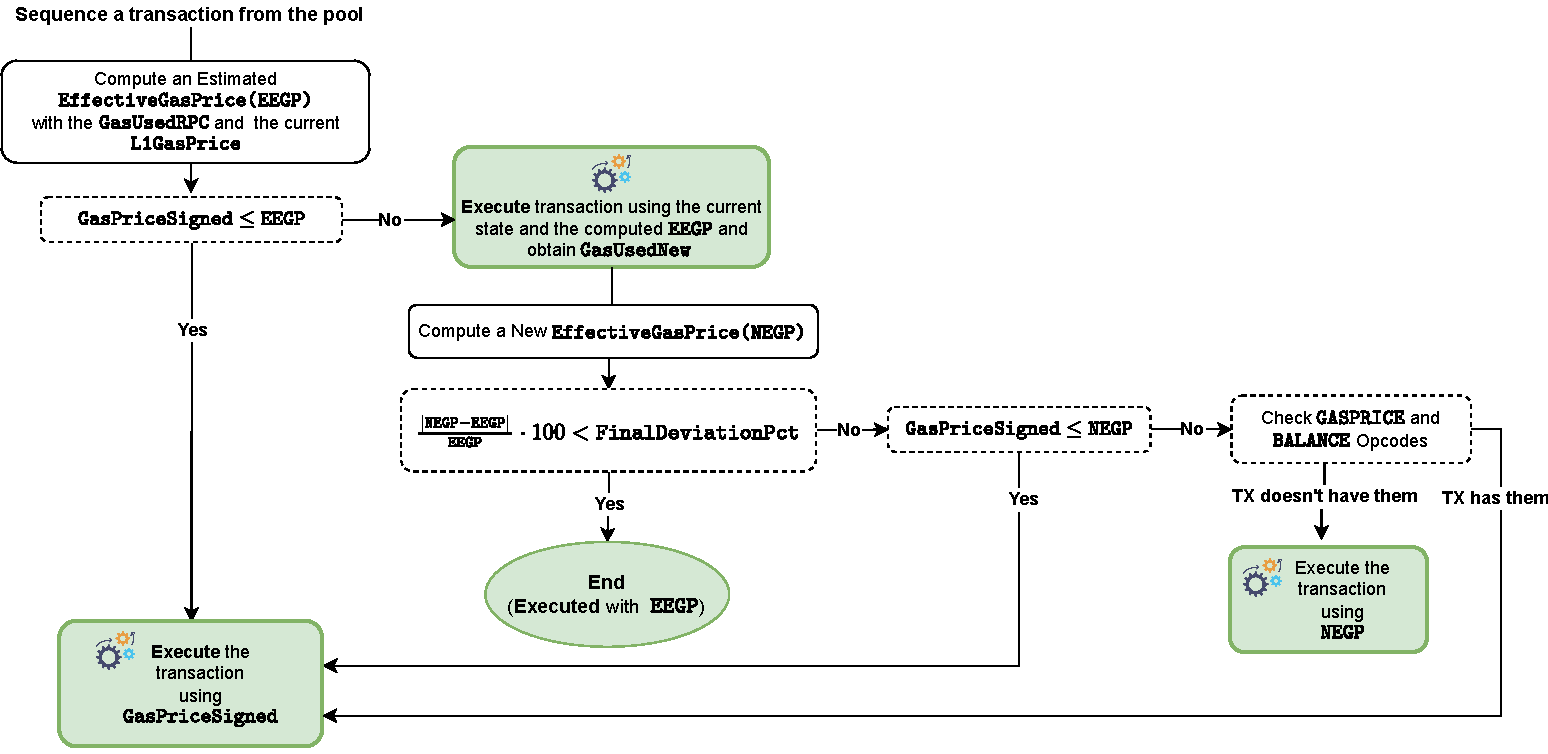
\includegraphics[width=0.9\textwidth]{\zkevmdir/figures/architecture/economics-users-fees/sequencer-diagram.drawio}
\caption{Flow of a transaction within the \textbf{Sequencer} component. Observe that we can not reject transactions at this point, so all of them should be included in the L1 State. }
\label{fig:sequencer-flow}
\end{figure}

\begin{enumerate}

\item The \textbf{Sequencer} computes the estimated \texttt{EffectiveGasPrice} (which we will call \texttt{EEGP}) using the \texttt{GasUsedRPC} obtained in the \textbf{RPC} pre-execution using a previous state root (which has now changed) and the current \texttt{L1GasPrice} (which also may differ from the one used when sending the transaction to the \textbf{RPC}) for all the transactions stored in the \textbf{Pool} and sequence the one having higher \texttt{EEGP}. It is important to note that this is done in this precise order. We could have calculated the \texttt{EEGP} just before storing the transactions in the \textbf{Pool} and sorting it by \texttt{EEGP}, but this would not yield the same result because the \texttt{L1GasPrice} at that moment is different from the one at the time of sequencing a transaction, potentially changing the \texttt{EEGP} as well as the prioritization order of transactions.

\item At this point, we have two options:

\begin{itemize}

\item If $\texttt{GasPriceSigned} \leq \texttt{EEGP}$, even with only an estimated effective gas price, there is a significant risk of loss. In such cases, we opt not to further adjust the gas price in order to reduce the number of executions needed to do so. Henceforth, the user is charged the full \texttt{GasPriceSigned}, so the \textbf{Executor} will execute the transaction using it, concluding the sequencing process.

\item Conversely, if $\texttt{GasPriceSigned} > \texttt{EEGP}$, there is a potential room for further adjustment for the gas price that will be charged to the user.

\end{itemize}

\item In the previous case, it is necessary to compute a more precise effective gas price based on the accurate amount of gas, denoted as \texttt{GasUsedNew}, obtained during the transaction's execution using the correct state root at the sequencing time (which was not known earlier for straightforward reasons). Henceforth, the \textbf{Executor} executes the transaction using \texttt{EEGP}, obtaining \texttt{GasUsedNew} which the sequencer utilizes to compute a new effective gas price referred to as \texttt{NEGP}.

\item We have to paths:

\begin{itemize}

\item If the percentage deviation between \texttt{EEGP} and \texttt{NEGP} is higher than a fixed deviation parameter \texttt{FinalDeviationPct} (which is $10$ in the actual configuration), that is
\[
\frac{\vert \texttt{NEGP} - \texttt{EEGP} \vert}{\texttt{EEGP}} \cdot 100 < \texttt{FinalDeviationParameter},
\]
indicates that there is minimal distinction between charging the user with \texttt{NEGP} compared to \texttt{EEGP}. Therefore, despite potential (but quite small) losses to the network or the user, we end up the flow just to avoid re-executions and save execution resources and we charge the user with \texttt{EEGP}.

\item On the contrary, if the percentage deviation equals or exceeds the deviation parameter
\[
\frac{\vert \texttt{NEGP} - \texttt{EEGP} \vert}{\texttt{EEGP}} \cdot 100 \geq \texttt{FinalDeviationParameter},
\]
there is a big difference between executions and we may better adjust gas price to potential (and quite big) losses to the network or the user.


\end{itemize}

\item In the later case, two options arise:

\begin{itemize}

\item If the gas price signed is less or equal than the accurate effective gas price computed with the correct state root
\[
\texttt{GasPriceSigned} \leq \texttt{NEGP},
\]
the network suffers again a risk of loss. Henceforth, the user is charged the full \texttt{GasPriceSigned}, so the \textbf{Executor} will execute the transaction using it, concluding the sequencing process.

\item Otherwise, if
\[
\texttt{GasPriceSigned} > \texttt{NEGP},
\]
means that we have margin to adjust the gas price that is charged to the user. However, in order to save executions and end up the adjustment process in this iteration, we will conclude the flow using a trick explained in the next point.

\end{itemize}

\item In the later case, we check if the transaction processing includes the two opcodes that use the gas price:

\begin{itemize}[-]

\item The \texttt{GASPRICE} opcode.

\item The \texttt{BALANCE} opcode from the source address.

\end{itemize}

We have two cases:

\begin{itemize}

\item If the transaction contains the aforementioned opcodes, we impose a penalty on the user for security reasons. In such cases, we simply proceed with executing the transaction using the entire \texttt{GasPriceSigned} to minimize potential losses and conclude the flow, as mentioned earlier. This precaution is employed to mitigate potential vulnerabilities in deployed Smart Contracts, that arise from creating a specific condition based on the gas price, for example, to manipulate execution costs.

\item If the transaction does not make use of the gas price-related opcodes, the \textbf{Executor} executes the transaction with the more adjusted gas price up to this point which is \texttt{NEGP} and end up the sequencing process.

\end{itemize}

\end{enumerate}



\subsection{Numerical Example: Sequencer Flow}


Let us continue the numerical example that has been carried during the whole document. In Figure \ref{fig:numerical-example-rpc} we represent, at the top of the timeline, the current \texttt{L1GasPrice} and, at the bottom, the associated $\texttt{GasPriceSuggested} = 0.15 \cdot \texttt{L1GasPrice}$ at the time of sequencing the transaction. Recall that in Section \ref{sec:numerical-example-rpc} we end up computing the \texttt{BreakEvenGasPriceRPC} of $2.52$ GWei/Gas.


\begin{figure}[H]
\centering
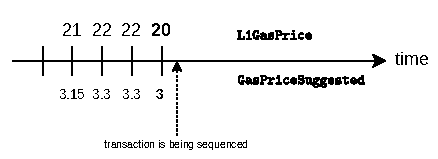
\includegraphics[width=0.7\textwidth]{\zkevmdir/figures/architecture/economics-users-fees/numerical-example-sequencer.drawio}
\caption{Timeline displaying the current \texttt{L1GasPrice} and its associated suggested gas price at the time of sequencing the transaction. }
\label{fig:numerical-example-sequencer}
\end{figure}


\begin{enumerate}

\item Imagine that the user signed a gas price of $3.3$ GWei/Gas. As illustrated in Figure \ref{fig:numerical-example-sequencer}, the network recommends a gas price of $3$ at the sequencing moment, equivalent to an L1 gas price of $20$. This results in an \texttt{EEGP} of
\[
\texttt{EEGP} = 2.722 \text{ GWei/Gas},
\]
where the $10$\% increase attributed to the prioritization carried out by \texttt{PriorityRatio} set at $0.1$.

\item Since the signed gas price is bigger than the estimated effective gas price
\[
\texttt{GasPriceSigned} = 3.3 > 2.772 = \texttt{EEGP},
\]
we execute the transaction using the current (and correct) state and the computed \texttt{EEGP} in order to obtain an accurate measure of the Gas used, which we call \texttt{GasUsedNew}. Suppose that, in this case, we obtain
\[
\texttt{GasUsedNew} = 95,000 \text{ Gas},
\]
which is bigger than the estimated gas of $60,000$ at the \textbf{RPC} pre-execution.

\item By using \texttt{GasUsedNew}, we can compute and adjusted effective gas price called \texttt{NEGP} as follows:
\begin{gather*}
\texttt{TxCostNew} = (200 \cdot 16 + 100 \cdot 4) \cdot 20 + 95,000 \cdot 20 \cdot 0.04 = 148,000 \text{ GWei}, \\
\texttt{BreakEvenGasPriceNew} = \frac{148,000}{95,000} \cdot 1.2 = 1.869 \text{ GWei/Gas}, \\
\texttt{NEGP} = 1.869 \cdot 1.1 = 2.056 \text{ GWei/Gas}.
\end{gather*}

Observe that the transaction cost is way higher than the estimated one of $126,000$ even when the L1 Gas Price has decreased from $21$ to $20$ due to a huge increase in Gas.

\item Observe that there is a significative deviation between both effective gas prices:
\[
\frac{\vert \texttt{NEGP} - \texttt{EEGP} \vert}{\texttt{EEGP}} \cdot 100 = 25.82 > 10.
\]
This deviation penalizes the user a lot since
\[
\texttt{GasPriceSigned} = 3.3 > 2.52 = \texttt{EEGP} \gg 2.056 = \texttt{NEGP},
\]
so we try to charge \texttt{NEGP} to the user to further adjust the gas price.

\item In this case, suppose that the transaction does not have neither \texttt{GASPRICE} nor \texttt{BALANCE} (from the source address) opcodes, so we will execute the transaction with
\[
\texttt{GasPriceFinal} = \texttt{NEGP} = 2.056 \text{ GWei/Gas}.
\]
Observe that \texttt{GasUsedFinal} should be the same as \texttt{GasUsedNew} $= 95,000$. We can now compute \texttt{EffectivePercentage} and \texttt{EffectivePercentageByte} as follows:
\begin{gather*}
\texttt{EffectivePercentage} = \frac{\texttt{GasPriceFinal}}{\texttt{GasPriceSigned}} = \frac{2.056}{3.3} = 0.623. \\
\texttt{EffectivePercentageByte} = \texttt{EffectivePercentage} \cdot 256  - 1 = 148.
\end{gather*}
Observe that the user has been charged with the $62.3$\% of the gas price he/she signed at the time of sending the transaction.

\end{enumerate}